% Created 2021-01-24 Sun 22:49
% Intended LaTeX compiler: pdflatex
\documentclass[11pt]{article}
\usepackage[utf8]{inputenc}
\usepackage[T1]{fontenc}
\usepackage{graphicx}
\usepackage{grffile}
\usepackage{longtable}
\usepackage{wrapfig}
\usepackage{rotating}
\usepackage[normalem]{ulem}
\usepackage{amsmath}
\usepackage{textcomp}
\usepackage{amssymb}
\usepackage{capt-of}
\usepackage{hyperref}
\usepackage{minted}
\hypersetup{colorlinks=true, linkcolor=black, filecolor=red, urlcolor=blue}
\usepackage[turkish]{babel}
\author{Eren Hatırnaz}
\date{22 Mart 2020}
\title{Yazılım Gündemi - 2020/11\\\medskip
\large 16-22 Mart 2020}
\hypersetup{
 pdfauthor={Eren Hatırnaz},
 pdftitle={Yazılım Gündemi - 2020/11},
 pdfkeywords={},
 pdfsubject={},
 pdfcreator={Emacs 27.1 (Org mode 9.3)},
 pdflang={Turkish}}
\begin{document}

\maketitle
\tableofcontents \clearpage\shorthandoff{=}

\begin{center}
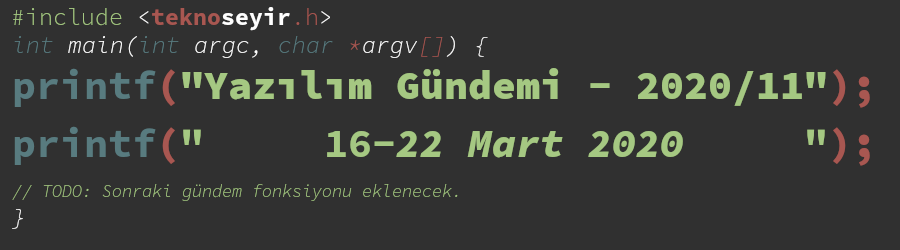
\includegraphics[width=.9\linewidth]{gorseller/yazilim-gundemi-banner.png}
\end{center}

\begin{center}
\href{../10/yazilim-gundemi-2020-10.pdf}{< Önceki Gündem} | \textbf{16-22 Mart 2020} | \href{../12/yazilim-gundemi-2020-12.pdf}{Sonraki Gündem >}

\href{https://teknoseyir.com/blog/yazilim-gundemi-2020-11}{TeknoSeyir'de Oku}
\end{center}

\section{GitHub, npm'i \href{https://github.blog/2020-03-16-npm-is-joining-github/}{satın aldı}}
\label{sec:orgc8c512f}
\begin{center}

\includegraphics[height=3cm]{gorseller/github-npm.png}
\end{center}

Aslında Microsoft satın aldı destek daha doğru olur. Çünkü GitHub da 2018
yılında Microsoft tarafından \href{https://techcrunch.com/2018/06/04/microsoft-has-acquired-github-for-7-5b-in-microsoft-stock/}{satın alınmıştı}. npm, front-end camiası için çok
önemli bir yere sahip. Her ne kadar Facebook tarafından geliştirilen \href{https://classic.yarnpkg.com/en/}{yarn} gibi
bir alternatifi olsa da hala daha npm pastanın büyük bir bölümünün sahibi.
Hatırladığım kadarıyla Windows'da NodeJS kurduğunuzda yanında otomatik olarak
npm de kurulu geliyordu. Değişti mi bilmiyorum ama npm'in bu kadar çok
kullanılmasının bir nedeni de budur. Öncesinde açık kaynak bir proje olarak
başlayan süreç zamanla şirketleşme yolundan devam etti ve bu hafta da GitHub
tarafından satın alındı.

GitHub'ın kendi sitesindeki blogunda yayınlanan yazı ile anlaşmanın
gerçekleştirildiği duyuruldu. Görebildiğim kadarıyla Microsoft'un GitHub'ı
satın aldığı zamanki kadar büyük tepkiler (insanlar github'dan depolarını
taşımaya başlamıştı) yok. Belki de dünyanın şu an çok farklı bir gündemi
olduğundan olabilir ama yine de \href{https://www.reddit.com/r/node/comments/fjocuy/npm\_is\_joining\_github\_and\_is\_now\_owned\_by/}{Reddit} ve \href{https://news.ycombinator.com/item?id=22594549}{HackerNews} gibi platformlarda
insanların tartışma konusu oldu.

Yazıdaki önemli bir nokta önümüzdeki senelerde GitHub Packages ve npm'in
Private Registry özelliklerinin birleştirilecek olması. Yani ücretli olarak
npm'in hizmetlerinden yararlananlar ilerleyen zamanlarda GitHub Packages'e
geçmeye zorlanabilirler.

Her ne kadar Microsoft'un son birkaç yıldır yaptığı açık kaynağa yatırım
işlerini beğeniyor olsam da bu kadar büyük iki geliştirici hizmeti ve aracının
tek bir firmanın elinde olması beni endişelendirmiyor değil. Bu konuda siz ne
düşünüyorsunuz? Yorumlar bölümünde konuşalım.
\section{GitHub Mobil, Beta \href{https://github.blog/2020-03-17-github-for-mobile-is-now-available/}{programından çıktı}}
\label{sec:org54dab42}
Geçtiğimiz sene kasım ayında düzenlenen GitHub Universe 2019 etkinliğinde
duyurulan GitHub Mobile Beta Program for iOS ve bu yılın başlarında duyurulan
GitHub Mobile Android Beta Program haberlerinden sonra sonunda GitHub'ın mobil
uygulamaları Beta'dan çıktı ve herkesin kullanımına açıldı.

Github Mobile uygulamasını indirmek için:
\begin{itemize}
\item Android: \url{https://play.google.com/store/apps/details?id=com.github.android}
\item iOS: \url{https://apps.apple.com/us/app/github/id1477376905}
\end{itemize}

\begin{center}
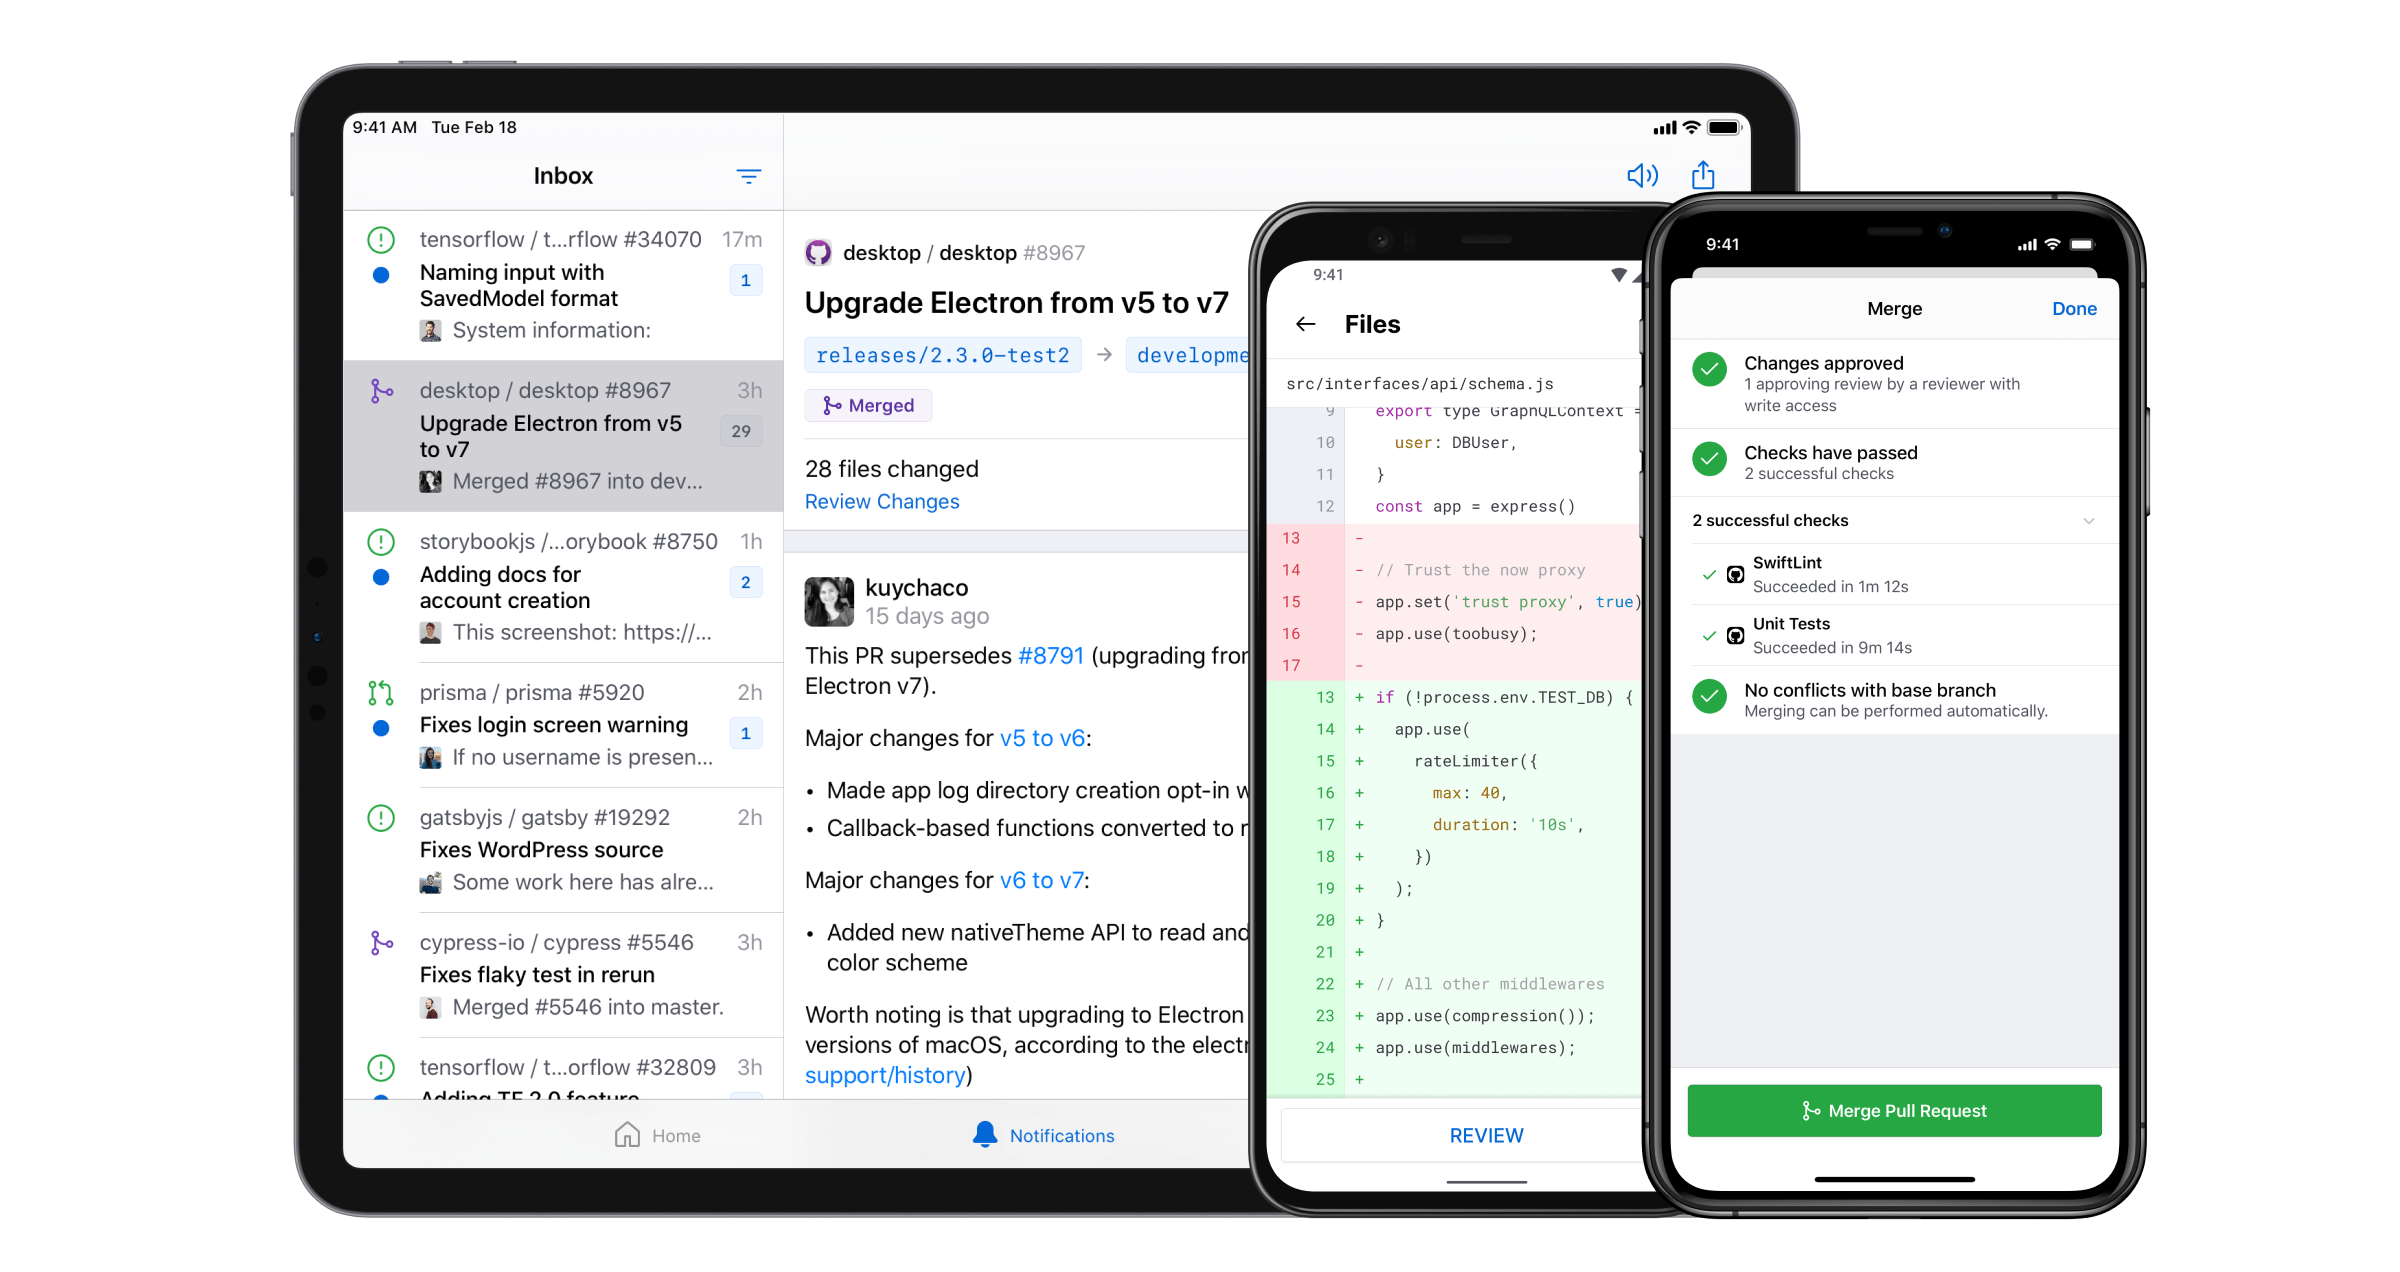
\includegraphics[width=.9\linewidth]{gorseller/github-mobile.png}
\end{center}

Daha önce iki işletim sistemi için de bu konuyu ele almıştık. Hatta ben direkt
iOS sistemindeki Beta programına kayıt olmuş ve kısa bir inceleme de yapmıştım
(bkz: \href{../../2019/18/yazilim-gundemi-18.pdf}{Yazılım Gündemi - 18}). Android için Beta programından da bu yılın ilk
yazılım gündemi yazılarında (bkz: \href{../03/yazilim-gundemi-03.pdf}{Yazılım Gündemi - 2020/03}) bahsetmiştim. Ben
iOS üzerindeki Beta programından kullanmaya devam ediyorum. GitHub'ın bu
eksikliği gidermesi güzel ama uygulamanın daha çok gelişmesi gerek. Örneğin şu
an sadece master branch'ı üzerindeki kodları görüntüleyebiliyoruz, branch
değiştirme özelliği uzun zamandır istenmesine rağmen henüz eklenmiş değil.
Bakalım, ben Beta programında kalmaya ve gelişmelerden sizleri haberdar etmeye
devam edeceğim.
\section{Github, "yanlışlıkla" popüler JavaScript framework'ü Aurelia'nın tüm depolarını kilitledi}
\label{sec:orgd41fcb6}
\begin{itemize}
\item \href{https://twitter.com/eisenbergeffect/status/1240671036292485121}{Konuyla ilgili Tweet}
\end{itemize}

Başlığa "popüler" yazmamın nedeni \href{https://github.com/aurelia/framework}{framework'ün ana deposu}nun yaklaşık 11.3K
star almış olması, yoksa ben de ismini ilk defa duyuyorum. Gerçekten ilginç
bir olay, Amerika merkezli bir şirket tarafından açık kaynak hale getirilmiş
bir yazılımın tüm GitHub depoları (\href{https://aurelia.io/}{Aurelia.io} sitesi de GitHub üzerinde host
ediliyormuş), yine Amerika'nın yaptırımları nedeniyle herkes için erişime
engelleniyor. Geliştiriciler ve katkı sağlayanlar kodlarına erişemiyor.

\begin{figure}[htbp]
\centering
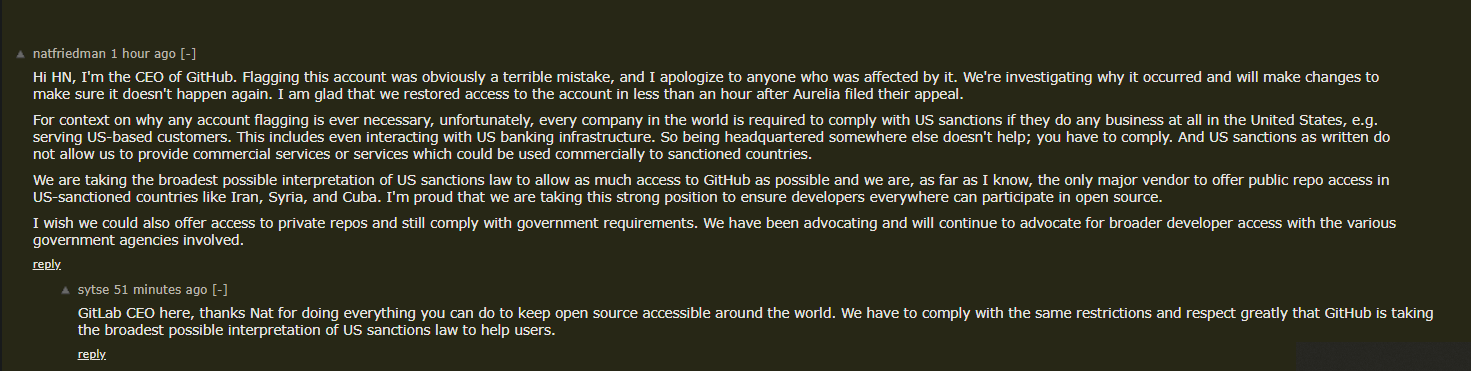
\includegraphics[width=.9\linewidth]{gorseller/github-ceo-hackernews.png}
\caption{GitHub CEO'unun \href{https://news.ycombinator.com/item?id=22628961}{HackerNews'deki konunun} altında yaptığı açıklama.}
\end{figure}

Her ne kadar olay birkaç saat içerisinde çözümlenmiş olsa da onlarca depo'nun
bu kadar bir "yanlışlık" nedeniyle erişime kapatılabiliyor olması beni rahatsız
etti. İlk yazılım gündemi yazılarının birinde (bkz: \href{../../2019/03/yazilim-gundemi-03.pdf}{Yazılım Gündemi - 3})
GitHub'ın, Amerika'nın ticari yaptırımlarını uygulamaya başladığından ve birçok
Kırım ve İran'lı geliştiricinin bu durumdan etkilendiğini konuşmuştuk. Ben
zaten o zamandan beri her ihtimale karşı tüm depolarımı bilgisayarıma
indirmiştim ve farklı yerlere yedeklemiştim ama bu vesile ile size tekrardan
hatırlamış olayım. Levent Abi'nin dediği gibi: "Bulut dediğin başkasının
bilgisayarıdır. Gün gelir de 'Sana hizmet vermiyorum kardeşim' derse, öylece
ortada kalırsın!"
\section{JDK 14 GA \href{https://jdk.java.net/14/}{yayınlandı}}
\label{sec:org667c6b5}
Geçtiğimiz aylar boyunca Release Candidate sürümleri yayınlanan JDK 14 sürümü
sonunda genel uygunluk (general availability) duruma geldi ve bu hafta
içerisinde yayınlandı. JDK 14 ile gelen birkaç özelliği incelleyelim.

\subsection{\href{https://openjdk.java.net/jeps/305}{JEP 305}: Pattern Matching for instanceof (Preview)}
\label{sec:org79a0b06}
Henüz ön-izleme durumunda olan bu özellik sayesinde aşağıdaki \texttt{instanceof}
kullanımı daha sade bir hal aldı.

\begin{minted}[breaklines=true,breakanywhere=true,frame=lines, linenos, label=Java]{java}
if (obj instanceof String) {
    String str = (String) obj;
    // str değişkeni ile işlemler
}
\end{minted}
Bu kullanım çok fazla yaygın fakat artık bu satırları aşağıdaki şekilde tek
satıra indirebileceğiz:
\begin{minted}[breaklines=true,breakanywhere=true,frame=lines, linenos, label=Java]{java}
if(obj instanceof String str) {
    // str burada kullanılabilir
} else {
    // str burada kullanılamaz
}
\end{minted}
\subsection{\href{https://openjdk.java.net/jeps/359}{JEP 356}: Records (Preview)}
\label{sec:org7aecd4f}
Java ya da nesne tabanlı herhangi bir dille biraz olsun haşır neşir
olmuşsanız aşağıdaki sınıf yapısı size de çok tanıdık gelecektir:
\begin{minted}[breaklines=true,breakanywhere=true,frame=lines, linenos, label=Java]{java}
public class Kisi {
    private String isim;
    private String soyisim;

    public Kisi(String isim, String soyisim) {
        this.isim = isim;
        this.soyisim = soyisim;
    }

    public String getIsim() {
        return this.isim;
    }

    public void setIsım(String isim) {
        this.isim = isim;
    }

    public String getSoyisim() {
        return this.soyisim;
    }

    public void setSoyisim(String soyisim) {
        this.soyisim = soyisim;
    }
}
\end{minted}
Gördüğünüz gibi basit bir kişi bilgisi tutmak için bile bu kadar kod yazmamız
gerekiyor (elbette bu yapının böyle olmasının çok doğru nedenleri mevcut) ama
bu JDK sürümü ile birlikte hayatımıza giren yeni tanımlama şeklide \texttt{Records}
ile yukarıdaki tüm kodları şu şekilde tek satıra indirebilirsiniz:
\begin{minted}[breaklines=true,breakanywhere=true,frame=lines, linenos, label=Java]{java}
record Kisi(String isim, String soyisim) { }
\end{minted}
Artık bunu da aynı sınıfmış gibi kullanabilirsiniz:
\begin{minted}[breaklines=true,breakanywhere=true,frame=lines, linenos, label=Java]{java}
Kisi eren = new Kisi("Eren", "Hatırnaz");

String isim = eren.isim();
String soyisim = eren.soyisim();
\end{minted}
Fakat bu özellim hem şu an ön-izleme durumunda, yani henüz çalışan
kodlarınıza eklemek için çok erken, hem de bazı kısıtlamaları var:
\begin{itemize}
\item Record kendisiyle birlikte içerisindeki tüm veri alanlarını 'final' olarak
işaretliyor. Dolayısıyla bu sınıfdan başka bir sınıf türetemiyor ve bir
obje oluşturduktan sonra değişkenleri üzerinde değişiklik yapamıyoruz.
\end{itemize}

Bunun gibi Record özelliğine ait diğer kurallar için alt konu başlığına
eklediğim bağlantıya tıklayabilir ya da Rahman Usta tarafından kodedu
sitesinde yazılmış \href{https://kodedu.com/2020/01/javada-recordlar/}{bu yazıyı} okuyabilirsiniz.

JDK 14 ile gelen diğer özellikler için konu başlığına eklediğim bağlantıya
tıklayabilir ya da 28 Mart tarihinde online olarak gerçekleşecek bu Webinere
kayıt olabilirsiniz: \href{https://istanbul-jug.org/2020/03/online-java-14-webineri/}{Online Java 14 Webineri - İstanbul Java User Group}.
\section{Eclipse 4.15 (2020-03) \href{https://www.eclipse.org/eclipse/news/4.15/}{sürümü yayınlandı}}
\label{sec:org4ac702e}
\begin{itemize}
\item \href{https://www.youtube.com/watch?v=XoUvOTiVaDc}{Konuyla ilgili YouTube videosu}
\end{itemize}

Eclipse 2020-03 sürümüne JDK 14 desteği eklemek için Eclipse Marketplace
üzerinden şu eklentiyi kurabilirsiniz: \href{https://marketplace.eclipse.org/content/java-14-support-eclipse-2020-03-415}{Java 14 Support for Eclipse 2020-03
(4.15)}
\section{.NET 5 Preview 1 \href{https://devblogs.microsoft.com/dotnet/announcing-net-5-0-preview-1/}{sürümü duyuruldu}}
\label{sec:org963410a}
Microsoft'un ".NET'in geleceği" olarak isimlendirdiği ve klasik .NET Framework
ile .NET Core'un birleşmiş hali .NET 5 sürümünün ilk ön-izleme sürümü bu hafta
içerisinde yayınlandı. Preview 1 ile birkaç performans iyileştirmesi de içeren
güncellemeler herkes tarafından erişilebilir durumda. Elbette production
ortamında çalışan uygulamalarınızı hemen geçirmek büyük risk olacaktır ama
kişisel projeleriniz için ufaktan kullanmaya ve Microsoft'a geri bildirim
göndermeye başlayabilirsiniz.
\section{Mozilla, Firefox'dan FTP \href{https://www.ghacks.net/2020/03/19/mozilla-will-remove-ftp-support-in-the-firefox-web-browser/}{desteğini kaldırıyor}}
\label{sec:org59fcd36}
2020 Haziran ayında yayınlanması planlanan Firefox 77 Stable sürümü ile
Mozilla takımı, Firefox içerisinden FTP desteğini "varsayılan olarak kapalı"
hale hale getirecek ve sonraki versiyonlarda ise desteği tamamen kaldırmayı
planlıyor. Tarayıcı üzerinden FTP kullanmak uzun zaman pek tercih edilen bir
şey değil zaten, o yüzden bu desteğin kalkacak olması çok da sürpriz olmadı.
Zaten Firefox 61 sürümüyle, web siteleri içerisinde yer alan \url{ftp://} uzaktılı
içerikleri (resim, müzik vb.) engellemişti. Firefox'un bu desteği
kaldırmasının ardında ise güvenlik sorunları yatıyor. FTP, kullanıcı adı ve
şifre dışında iletişimle ilgili bir güvenlik katmanı barındırmayan bir
protokol olduğu için trafik kolayca izlenebiliyor. Google'un Chrome tarayıcısı
da aynı şekilde desteğini sonlandırmaya hazırlanıyor. O da tarayıcıdaki ftp
uzantılı bağlantıları sistemde yüklü olan ftp istemcisine yönlendirecek. Bir
mail adresine tıkladığınız Outlook vb. programların açılması gibi.

\begin{figure}[htbp]
\centering
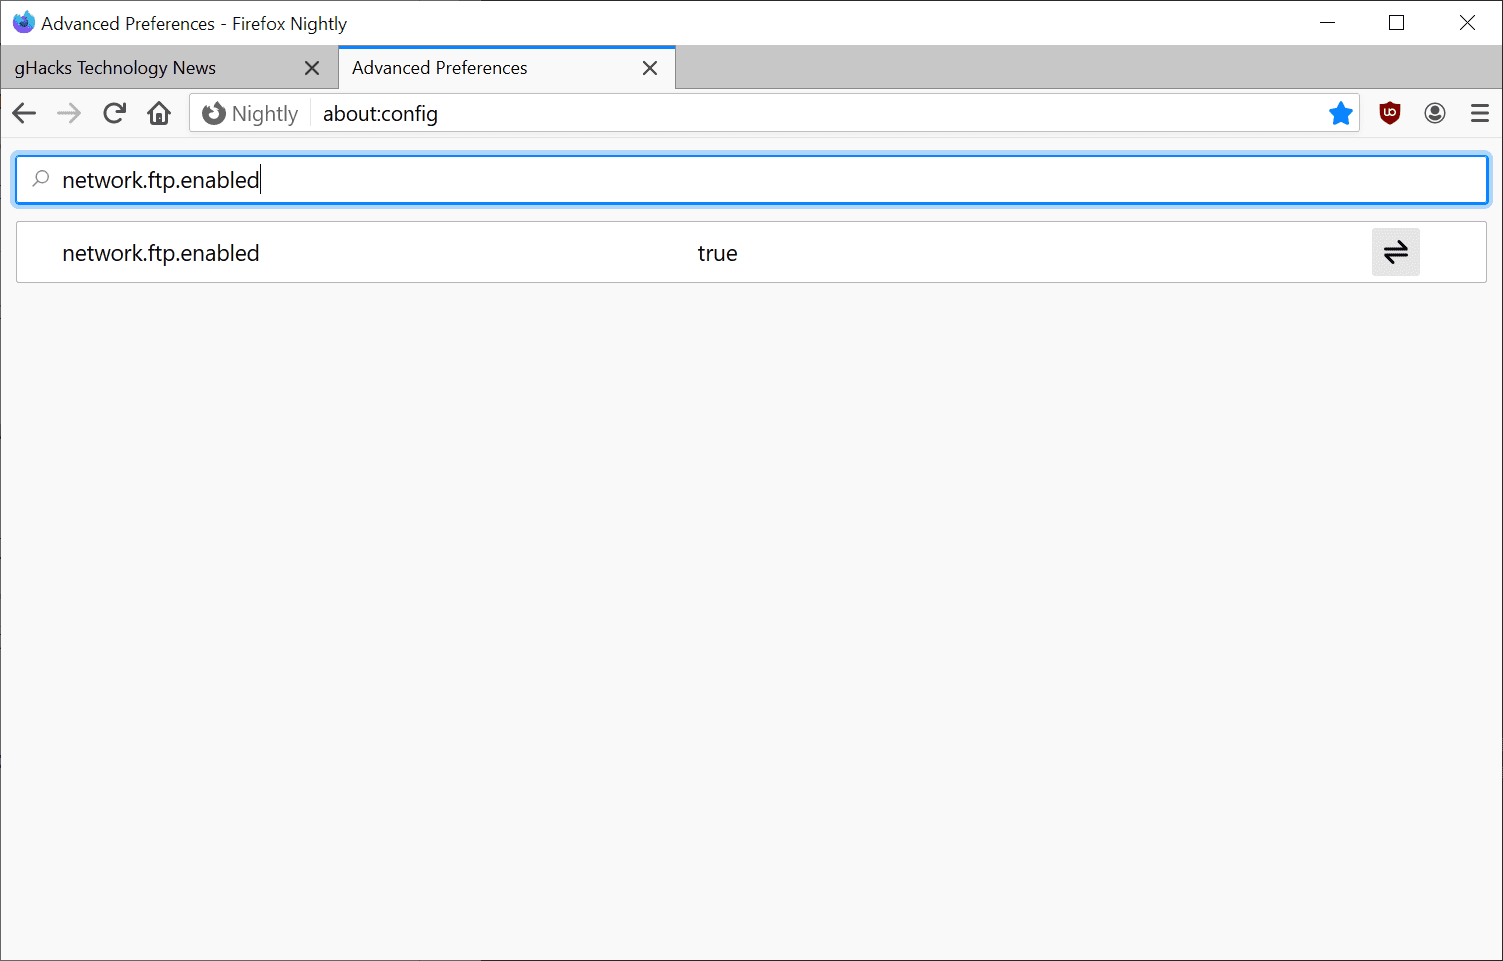
\includegraphics[width=.9\linewidth]{gorseller/firefox-ftp.png}
\caption[\texttt{network.ftp.enabled}]{Yine de Firefox üzerinde ftp kullanmakta ısrarcıysanız about:config sayfasına girip, \texttt{network.ftp.enabled} değişkenini true olarak değiştirebilirsiniz}
\end{figure}

Ayrıca bu hafta içerisinde ilginç de bir olay gerçekleşti: Coronavirüs
nedeniyle Firefox ve Chrome, \href{https://www.ghacks.net/2020/03/21/mozilla-re-enables-tls-1-0-and-1-1-because-of-coronavirus-and-google/}{TLS 1.0 ve TLS 1.1'e tekrar destek vermeye
başladı}. HTTPS bağlantıların gerçeklemesini sağlayan TLS protokolünün bu eski
sürümleri aslında iki tarayıcıdan da kaldırılmıştı fakat bu hafta içerisinde bu
değişiklikler geri alındı. Çünkü bazı devlet siteleri hala daha eski
protokolleri kullandığı için kullanıcıların erişememesi söz konusu olabilirdi.
Coronavirüs gündemdeyken bu tarz protokol versiyonu yükseltme işleri de öncelik
kapsamında olmadığı için Firefox ve Chrome'da böyle bir şey yapma gereği duydu.

\begin{figure}[htbp]
\centering
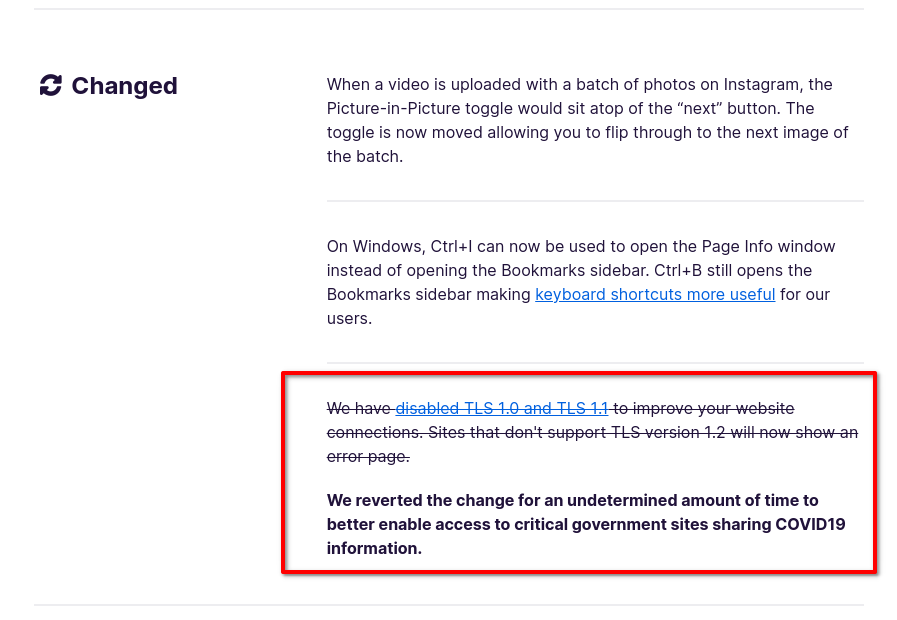
\includegraphics[width=.9\linewidth]{gorseller/firefox-chrome-tls10-11.png}
\caption{Firefox 74.0 sürümünün değişiklik notları sayfasındaki geri alma duyurusu}
\end{figure}
\newpage
\section{Windows Terminal Preview v0.10 \href{https://devblogs.microsoft.com/commandline/windows-terminal-preview-v0-10-release/}{sürümü yayınlandı}}
\label{sec:org5c87889}
Microsoft'un Terminal takımı geliştirmelere devam ediyor. Bu hafta yayınlanan
sürümle birlikte Windows'un yeni terminal uygulamasının ön-izleme v0.10
sürümüne fare desteği eklendi. Artık destekleyen konsol uygulamaları üzerinde
fare ile de giriş yapılabilecek.

\url{gorseller/windows-terminal-fare.gif}

Eklenen diğer özellik ve geliştirmeler için konu başlığına eklediğim
bağlantıya tıklayabilirsiniz.
\section{Diğer Haberler}
\label{sec:org09f9ee7}
\begin{itemize}
\item Koronavirüs nedeniyle iptal edilen ve ertelenen etkinlikler:
\begin{itemize}
\item Google Cloud Next '20: Digital Connect \href{https://cloud.google.com/blog/topics/inside-google-cloud/postponing-google-cloud-next20-digital-connect}{etkinliği ertelendi}.
\item Google I/O 2020 \href{https://www.theverge.com/2020/3/20/21188669/google-i-o-canceled-2020-coronavirus-pandemic}{tamamen iptal edildi}.
\item PyCon US 2020 \href{https://pycon.blogspot.com/2020/03/pycon-us-2020-in-pittsburgh.html?m=1}{iptal edildi}.
\end{itemize}
\item Visual Studio 2019 version 16.5 \href{https://devblogs.microsoft.com/visualstudio/visual-studio-2019-version-16-5/}{yayınlandı}.
\item Facebook, kendi tarih-saat \href{https://engineering.fb.com/production-engineering/ntp-service/}{sunucularını açtı}.
\item Docker'a GitHub Actions \href{https://www.docker.com/blog/first-docker-github-action-is-here/}{desteği geldi}.
\item DirectX 12 Ultimate \href{https://devblogs.microsoft.com/directx/announcing-directx-12-ultimate/}{sürümü yayınlandı}.
\item Prettier aracının 2.0 \href{https://prettier.io/blog/2020/03/21/2.0.0.html}{sürümü yayınlandı}.
\item PHP programlama dilinin 3 ayrı sürümüne güncelleme geldi:
\begin{itemize}
\item PHP 7.4.4 \href{https://www.php.net/ChangeLog-7.php\#7.4.4}{yayınlandı}.
\item PHP 7.3.16 \href{https://www.php.net/ChangeLog-7.php\#7.3.16}{yayınlandı}.
\item PHP 7.2.29 \href{http://www.php.net/ChangeLog-7.php\#7.2.29}{yayınlandı}.
\end{itemize}
\item D programlama dilinin 2.091.0 \href{https://dlang.org/blog/2020/03/17/d-2-091-0-released/}{sürümü yayınlandı}.
\item Julia programlama dilinin v1.4.0 \href{https://discourse.julialang.org/t/julia-v1-4-0-has-been-released/36324}{sürümü yayınlandı}.
\item TensorFlow 2.2.0-rc1 \href{https://github.com/tensorflow/tensorflow/releases/tag/v2.2.0-rc1}{sürümü yayınlandı}.
\item \href{https://streamnative.io/blog/tech/2020-03-17-announcing-the-apache-pulsar-2020-user-survey-report/}{Apache Pulsar 2020 Kullanıcı Anketi Raporu} yayınlandı.
\item GraphQLize Alpha \href{https://www.graphqlize.org/blog/announcing-graphqlize-alpha/}{duyuruldu}.
\item Yeni bir Racket kütüphanesi \href{https://dedbox.github.io/2020/03/template-macros-initial-release.html}{duyuruldu}: \href{https://github.com/dedbox/racket-template}{Template Macros}.
\item Tokie aracının 11.0 \href{https://github.com/XAMPPRocky/tokei/releases/tag/v11.0.0}{sürümü yayınlandı}.
\item Ionic CLI aracının 6.3.0 \href{https://github.com/ionic-team/ionic-cli/releases/tag/\%2540ionic\%252Fcli\%25406.3.0}{sürümü yayınlandı}.
\end{itemize}
\section{Lisans}
\label{sec:org55f6eaf}
\begin{center}
\begin{center}

\includegraphics[height=1.5cm]{../../../img/CC_BY-NC-SA_4.0.png}
\end{center}

\href{yazilim-gundemi-2020-11.pdf}{Yazılım Gündemi - 2020/11} yazısı \href{https://erenhatirnaz.github.io}{Eren Hatırnaz} tarafından \href{http://creativecommons.org/licenses/by-nc-sa/4.0/}{Creative Commons
Atıf-GayriTicari-AynıLisanslaPaylaş 4.0 Uluslararası Lisansı} (CC BY-NC-SA 4.0)
ile lisanslanmıştır.
\end{center}
\end{document}
